\documentclass[11pt,a4paper]{article}

% --- Packages ---
\usepackage[utf8]{inputenc}
\usepackage[margin=1in]{geometry}
\usepackage{amsmath, amssymb, amsfonts, amsthm}
\usepackage{graphicx}
\usepackage{booktabs}
\usepackage{xcolor}
\usepackage{listings}
\usepackage{fancyhdr}
\usepackage{titlesec}
\usepackage{setspace}
\usepackage{tcolorbox}
\usepackage{hyperref}
\usepackage{float}
\usepackage{tabularx}
\usepackage{microtype}
\usepackage{tikz}
\usetikzlibrary{arrows.meta, calc, positioning}

% --- Typography (Palatino Serif + Helvetica Sans + Courier Monospace) ---
\usepackage[sc]{mathpazo}
\usepackage[scaled=0.95]{helvet}
\usepackage{courier}

% --- Custom Tabularx Column Types ---
\newcolumntype{C}{>{\centering\arraybackslash}X}
\newcolumntype{L}{>{\raggedright\arraybackslash}X}
\newcolumntype{R}{>{\raggedleft\arraybackslash}X}

% --- Color Palette (Corporate Blue Theme) ---
\definecolor{NavyBlue}{RGB}{11, 47, 100}
\definecolor{SlateGray}{RGB}{70, 80, 95}
\definecolor{TealAccent}{RGB}{0, 102, 102}
\definecolor{LightBG}{RGB}{247, 249, 252}
\definecolor{CodeGreen}{RGB}{0, 120, 0}
\definecolor{CodePurple}{RGB}{128, 0, 128}
\definecolor{Charcoal}{RGB}{34, 34, 34}

% --- Custom Page Layout ---
\pagestyle{fancy}
\fancyhf{}
\fancyhead[L]{\color{SlateGray}\small CSE 406: Cyber Security Sessional --- Assignment 1}
\fancyhead[R]{\color{SlateGray}\small Student ID: 2105032}
\fancyfoot[C]{\color{SlateGray}\thepage}
\renewcommand{\headrulewidth}{0.4pt}
\renewcommand{\footrulewidth}{0pt}

% --- Section Styling ---
\titleformat{\section}
  {\color{NavyBlue}\normalfont\Large\bfseries}
  {\thesection}{1em}{}[\titlerule]
\titleformat{\subsection}
  {\color{NavyBlue}\normalfont\large\bfseries}
  {\thesubsection}{1em}{}
\titleformat{\subsubsection}
  {\color{NavyBlue}\normalfont\normalsize\bfseries}
  {\thesubsubsection}{1em}{}

% --- Code Listing Styling ---
\lstdefinestyle{pythonstyle}{
    backgroundcolor=\color{LightBG},   
    commentstyle=\color{CodeGreen}\itshape,
    keywordstyle=\color{NavyBlue}\bfseries,
    numberstyle=\tiny\color{SlateGray},
    stringstyle=\color{CodePurple},
    basicstyle=\ttfamily\footnotesize\color{Charcoal},
    breakatwhitespace=false,         
    breaklines=true,                 
    captionpos=b,                    
    keepspaces=true,                 
    numbers=left,                    
    numbersep=8pt,                  
    showspaces=false,                
    showstringspaces=false,
    showtabs=false,                  
    tabsize=4,
    frame=single,
    rulecolor=\color{SlateGray!30},
    keywordstyle=[2]\color{TealAccent}\bfseries,
    keywords=[2]{Sbox,InvSbox,Rcon,Mixer,InvMixer,gf_mult,GF_LUT}
}
\lstset{style=pythonstyle}

% --- Hyperref Setup ---
\hypersetup{
    colorlinks=true,
    linkcolor=NavyBlue,
    filecolor=TealAccent,      
    urlcolor=TealAccent,
    citecolor=NavyBlue
}

% --- Paragraph Formatting ---
\setstretch{1.15}
\setlength{\parskip}{0.5em}
\setlength{\parindent}{0pt}

% --- Custom Math Operators ---
\DeclareMathOperator{\GF}{GF}

\begin{document}

% =========================================================================
% TITLE PAGE
% =========================================================================
\begin{titlepage}
    \pagenumbering{Alph}
    \thispagestyle{empty}
    \centering
    \vspace*{0.2cm}
    
    
\includegraphics[width=2.5cm]{images/BUET_logo_256px_color.png}\\
    \vspace{0.4cm}
    
    {\Huge\bfseries\color{NavyBlue} Department of Computer Science and Engineering\\}
    {\Large\bfseries\color{SlateGray} Bangladesh University of Engineering and Technology (BUET)\\}
    
    \vspace{1.0cm}
    \rule{\linewidth}{1.5pt}
    \begin{tcolorbox}[colback=NavyBlue!5!white, colframe=NavyBlue, arc=4pt, boxrule=1.5pt, left=15pt, right=15pt, top=15pt, bottom=15pt]
        \centering
        \vspace{0.2cm}
        {\Huge\bfseries\color{NavyBlue} Offline-1: AES + Diffie-Hellman Cryptosystem\\}
        \vspace{0.3cm}
        {\Large\bfseries\color{SlateGray} Design, Theory, and Performance Analysis of an End-to-End Symmetric-Key Hybrid Cryptosystem\\}
        \vspace{0.2cm}
    \end{tcolorbox}
    \rule{\linewidth}{1.5pt}
    
    \vspace{1.0cm}
    
    \begin{tabular}{ll}
        \textbf{Course Title:} & CSE 406 --- Cyber Security Sessional \\
        \textbf{Academic Term:} & Level 4, Term 1 (January 2026) \\
        \textbf{Assignment Reference:} & Offline-1 (Cryptography) \\
    \end{tabular}
    
    \vspace{1.2cm}
    
    \begin{tcolorbox}[colback=LightBG, colframe=SlateGray!40, arc=2pt, boxrule=0.5pt, width=0.6\textwidth]
        \centering
        \textbf{Submitted By:}\\
        \vspace{0.2cm}
        {\large\bfseries Nawriz Ahmed Turjo}\\
        Student ID: \textbf{2105032}\\
        Section: A2
    \end{tcolorbox}
    
    \vfill
    {\color{SlateGray}\large Submitted on: July 14, 2026}
\end{titlepage}

\newpage
\thispagestyle{empty}
\pagenumbering{roman}

% =========================================================================
% TABLE OF CONTENTS
% =========================================================================
\tableofcontents
\newpage
\pagenumbering{arabic}

% =========================================================================
% SECTION 1: INTRODUCTION
% =========================================================================
\section{Introduction}
Modern information security relies heavily on \textbf{hybrid cryptosystems} to balance safety and performance. While public-key (asymmetric) cryptosystems solve the primary bottleneck of secure key transport over insecure networks, they are computationally intensive. Conversely, symmetric-key ciphers are orders of magnitude faster but require a pre-shared secret key. 

This project details the independent implementation of a secure symmetric-key hybrid cryptosystem from first principles:
\begin{enumerate}
    \item \textbf{Diffie-Hellman Key Exchange}: A secure, modular arithmetic key-exchange protocol executed over a TCP socket channel, enabling two untrusted endpoints (\textbf{Alice} and \textbf{Bob}) to establish a shared cryptographic secret.
    \textbf{Miller-Rabin primality testing} and \textbf{safe prime generators} ensure resistance to discrete logarithm attacks.
    \item \textbf{Advanced Encryption Standard (AES)}: A symmetric block cipher implementation executing the standard round transformations ($SubBytes$, $ShiftRows$, $MixColumns$, and $AddRoundKey$) in column-major order to achieve strong confusion and diffusion properties.
    \item \textbf{Modes of Operation \& Transport}: Encryption and decryption of multi-block messages in both \textbf{Electronic Codebook (ECB)} and \textbf{Cipher Block Chaining (CBC)} configurations (with proper \textbf{PKCS\#7 padding}), streaming textual payloads and arbitrary binary files over network interfaces.
\end{enumerate}

The system components are implemented natively in Python without relying on high-level cryptography suites (using only low-level math primitives and helper constants for finite field mappings). 

\subsection{End-to-End System Architecture}
To illustrate the interaction between the sender (\textbf{Alice}) and the receiver (\textbf{Bob}), the following sequence mapping outlines the hybrid system lifecycle:

\begin{enumerate}
    \item \textbf{Parameter Generation (Step 1)}: Alice generates public parameters locally using Miller-Rabin testing to produce a safe prime $P$ (where $P = 2q + 1$ and $q$ is prime) and finding a generator $g$ for the multiplicative subgroup of order $q$.
    \item \textbf{Key Exchange (Step 2)}: Alice generates a private exponent $K_a$, computes public key $A = g^{K_a} \bmod P$, and transmits the tuple $(P, g, A)$ over the TCP socket. Bob accepts, generates his private exponent $K_b$, computes public key $B = g^{K_b} \bmod P$, and transmits $B$ back to Alice.
    \item \textbf{Key Derivation (Step 3)}: Both parties calculate the shared secret $s$ independently:
    \begin{equation}
        s = B^{K_a} \bmod P \quad (\text{Alice}) \quad \text{and} \quad s = A^{K_b} \bmod P \quad (\text{Bob})
    \end{equation}
    A 128-bit session key $K$ is derived from $s$ by taking its big-endian byte representation.
    \item \textbf{Secure Session Transmission (Step 4)}: Alice encrypts the payload (text or binary file bytes) in CBC mode using $K$ and a randomly generated IV. She formats the transmission using a 4-part protocol header frame:
    \begin{equation*}
        \mathtt{[Message\ Type:\ 4B]} \parallel \mathtt{[Filename\ Length:\ 4B]} \parallel \mathtt{[Filename:\ Var]} \parallel \mathtt{[Ciphertext\ Length:\ 10B]}
    \end{equation*}
    The ciphertext stream is sent once Bob signals he is \texttt{"READY"}. Bob receives the header, reads the expected ciphertext length, decrypts the block, and strips the PKCS\#7 padding.
\end{enumerate}

The sequence flow is visualized in Figure~\ref{fig:seq_diag}.

\begin{figure}[H]
    \centering
    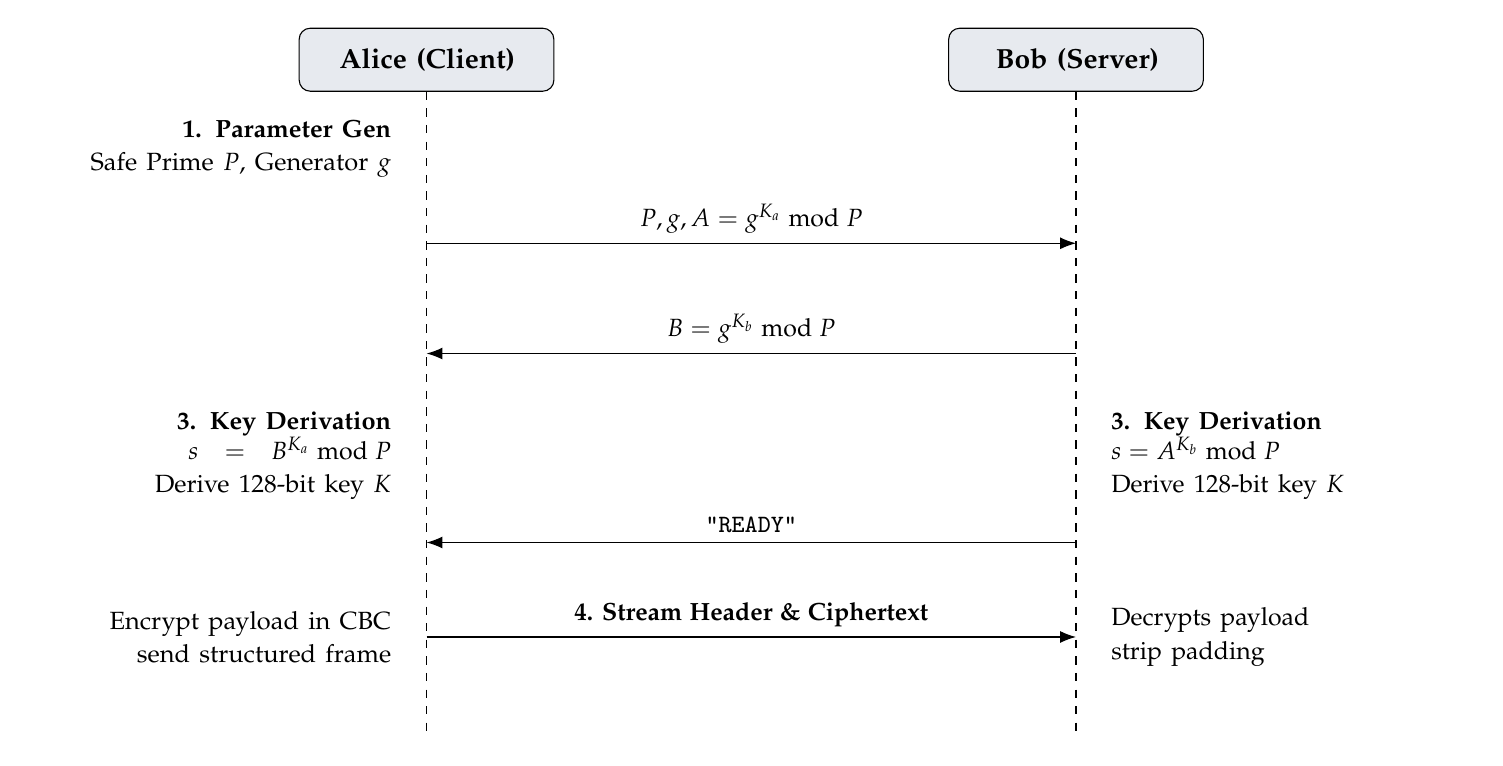
\begin{tikzpicture}[
        node distance = 1.2cm and 2.5cm,
        box/.style = {draw, fill=LightBG, text width=3cm, align=center, minimum height=0.8cm, rounded corners},
        line/.style = {draw, -{Latex[scale=1.2]}},
        dashline/.style = {draw, dashed}
    ]
        % Lifelines
        \node (alice_node) [box, fill=NavyBlue!10] {\textbf{Alice (Client)}};
        \node (bob_node) [box, fill=NavyBlue!10, right=5cm of alice_node] {\textbf{Bob (Server)}};
        
        \draw [dashline] (alice_node.south) -- ($(alice_node.south) - (0,8.2cm)$);
        \draw [dashline] (bob_node.south) -- ($(bob_node.south) - (0,8.2cm)$);
        
        % Step 1: Parameter Gen
        \node (step1) [below=0.6cm of alice_node.south] {};
        \node [left=0.2cm of step1, text width=4cm, align=right] {\small \textbf{1. Parameter Gen}\\ Safe Prime $P$, Generator $g$};
        
        % Step 2: DH Alice to Bob
        \node (step2a) [below=1.8cm of alice_node.south] {};
        \node (step2b) [below=1.8cm of bob_node.south] {};
        \draw [line] (step2a.center) -- (step2b.center) node [midway, above] {\small $P, g, A = g^{K_a} \bmod P$};
        
        % Step 2: DH Bob to Alice
        \node (step3a) [below=3.2cm of alice_node.south] {};
        \node (step3b) [below=3.2cm of bob_node.south] {};
        \draw [line] (step3b.center) -- (step3a.center) node [midway, above] {\small $B = g^{K_b} \bmod P$};
        
        % Step 3: Key Derivation
        \node (step4a) [below=4.5cm of alice_node.south] {};
        \node (step4b) [below=4.5cm of bob_node.south] {};
        \node [left=0.2cm of step4a, text width=4.5cm, align=right] {\small \textbf{3. Key Derivation}\\ $s = B^{K_a} \bmod P$\\ Derive 128-bit key $K$};
        \node [right=0.2cm of step4b, text width=4.5cm, align=left] {\small \textbf{3. Key Derivation}\\ $s = A^{K_b} \bmod P$\\ Derive 128-bit key $K$};
        
        % Bob ready
        \node (step5a) [below=5.6cm of alice_node.south] {};
        \node (step5b) [below=5.6cm of bob_node.south] {};
        \draw [line] (step5b.center) -- (step5a.center) node [midway, above] {\small \texttt{"READY"}};

        % Step 4: Secure Session
        \node (step6a) [below=6.8cm of alice_node.south] {};
        \node (step6b) [below=6.8cm of bob_node.south] {};
        \draw [line] (step6a.center) -- (step6b.center) node [midway, above] {\small \textbf{4. Stream Header \& Ciphertext}};
        \node [left=0.2cm of step6a, text width=4cm, align=right] {\small Encrypt payload in CBC\\ send structured frame};
        \node [right=0.2cm of step6b, text width=4.5cm, align=left] {\small Decrypts payload\\ strip padding};
        
    \end{tikzpicture}
    \caption{End-to-End Hybrid Cryptosystem Sequence Flow Diagram.}
    \label{fig:seq_diag}
\end{figure}

\newpage

% =========================================================================
% SECTION 2: THEORETICAL BACKGROUND
% =========================================================================
\section{Theoretical Background and Mathematical Formulations}

\subsection{Diffie-Hellman Key Exchange Protocol}
The Diffie-Hellman (DH) protocol relies on the computational difficulty of the \textbf{Discrete Logarithm Problem (DLP)} in multiplicative groups of finite fields. Given the public values $g^x \bmod P$, $g$, and $P$, determining the exponent $x$ is computationally infeasible for a sufficiently large prime $P$.

\subsubsection{Protocol Execution Flow}
Alice and Bob negotiate parameters publicly and compute key values:
\begin{enumerate}
    \item \textbf{Parameter Setup}: A large prime $P$ and a generator $g$ of the multiplicative group $\mathbb{Z}_P^*$ (where $1 < g < P$) are generated.
    \item \textbf{Private/Public Key Generation}:
    \begin{itemize}
        \item Alice generates a random secret exponent $K_a \ge k$-bits and computes:
        \begin{equation}
            A = g^{K_a} \bmod P
        \end{equation}
        \item Bob generates a random secret exponent $K_b \ge k$-bits and computes:
        \begin{equation}
            B = g^{K_b} \bmod P
        \end{equation}
    \end{itemize}
    \item \textbf{Key Negotiation}: Alice transmits $A$ to Bob, and Bob transmits $B$ to Alice.
    \item \textbf{Shared Secret Derivation}:
    \begin{itemize}
        \item Alice computes:
        \begin{equation}
            s = B^{K_a} \bmod P
        \end{equation}
        \item Bob computes:
        \begin{equation}
            s = A^{K_b} \bmod P
        \end{equation}
    \end{itemize}
    Both compute the same value because:
    \begin{equation}
        s = (g^{K_b})^{K_a} \equiv (g^{K_a})^{K_b} \equiv g^{K_a K_b} \pmod{P}
    \end{equation}
\end{enumerate}

\subsubsection{Miller-Rabin Primality Testing}
To guarantee that $P$ is prime, a probabilistic primality test is used. The Miller-Rabin test begins by writing $P-1$ as:
\begin{equation}
    P - 1 = 2^s \cdot d \quad \text{where } d \text{ is odd}
\end{equation}
For a chosen base $a \in [2, P-2]$, we check if:
\begin{equation}
    a^d \equiv 1 \pmod{P} \quad \text{or} \quad a^{2^r \cdot d} \equiv P - 1 \pmod{P} \quad \text{where } r \in [0, s-1]
\end{equation}
If neither condition holds, the candidate $P$ is composite. Repeating this check with $N$ independent random bases reduces the false-positive probability to less than $4^{-N}$. For security, $N = 40$ iterations were selected.

\subsubsection{Safe Prime Criteria and Generator Selection}
A prime $P$ is a \textbf{safe prime} if it satisfies:
\begin{equation}
    P = 2q + 1
\end{equation}
where $q$ is also prime (a Sophie Germain prime). Using a safe prime prevents attacks like the \textbf{Pohlig-Hellman algorithm}, which exploits prime factors of $P-1$. In a safe prime, $P-1 = 2q$, meaning the only prime factors of $P-1$ are $2$ and $q$.

To find a generator $g \in [2, P-2]$ for the subgroup of order $q$ or $2q$ in $\mathbb{Z}_P^*$, we ensure that for all prime factors $r$ of $P-1$:
\begin{equation}
    g^{(P-1)/r} \not\equiv 1 \pmod{P}
\end{equation}
Since the only prime factors of $P-1$ are $\{2, q\}$, generator validation simplifies to testing:
\begin{equation}
    g^2 \not\equiv 1 \pmod{P} \quad \text{and} \quad g^q \not\equiv 1 \pmod{P}
\end{equation}
If $g$ meets both criteria, it is confirmed as a valid generator.

\subsection{Advanced Encryption Standard (AES)}
AES is a symmetric-key block cipher that operates on a \textbf{4 $\times$ 4 state matrix} of bytes in column-major order.
Let a 16-byte block be $B = [b_0, b_1, \dots, b_{15}]$. The state matrix $S$ is organized as:
\begin{equation}
    S = \begin{bmatrix}
        b_0 & b_4 & b_8 & b_{12} \\
        b_1 & b_5 & b_9 & b_{13} \\
        b_2 & b_6 & b_{10} & b_{14} \\
        b_3 & b_7 & b_{11} & b_{15}
    \end{bmatrix}
\end{equation}

\subsubsection{Finite Field Arithmetic in \texorpdfstring{$\GF(2^8)$}{GF(2\textasciicircum 8)}}
AES addition and multiplication are performed in the Galois Field $\GF(2^8)$ defined by the irreducible polynomial:
\begin{equation}
    P(x) = x^8 + x^4 + x^3 + x + 1
\end{equation}
\begin{itemize}
    \item \textbf{Addition}: Addition of two byte values $A(x) + B(x)$ corresponds to the bitwise exclusive-OR (XOR) operation:
    \begin{equation}
        A \oplus B
    \end{equation}
    \item \textbf{Multiplication}: Multiplication of $A(x) \cdot B(x)$ is computed modulo $P(x)$. This is performed efficiently using binary shifts and reductions, known as the \textbf{xtime} operation:
    \begin{equation}
        x \cdot A(x) \pmod{P(x)} = \begin{cases}
            A(x) \ll 1 & \text{if the MSB of } A \text{ is } 0 \\
            (A(x) \ll 1) \oplus \mathtt{0x1B} & \text{if the MSB of } A \text{ is } 1
        \end{cases}
    \end{equation}
\end{itemize}

\subsubsection{Round Transformations}
Each intermediate round $i \in [1, N_r-1]$ consists of four steps:
\begin{enumerate}
    \item \textbf{SubBytes}: A non-linear byte substitution. Each byte $S_{r,c}$ in the state is mapped to its multiplicative inverse in $\GF(2^8)$, followed by an affine transformation over $\GF(2)$:
    \begin{equation}
        S_{r,c} \leftarrow \mathtt{Sbox}[S_{r,c}]
    \end{equation}
    \item \textbf{ShiftRows}: A cyclic shift applied to the rows of the state. Row $r$ (indexed $0 \le r \le 3$) is cyclically shifted left by $r$ bytes:
    \begin{equation}
        \begin{bmatrix}
            s_{0,0} & s_{0,1} & s_{0,2} & s_{0,3} \\
            s_{1,0} & s_{1,1} & s_{1,2} & s_{1,3} \\
            s_{2,0} & s_{2,1} & s_{2,2} & s_{2,3} \\
            s_{3,0} & s_{3,1} & s_{3,2} & s_{3,3}
        \end{bmatrix}
        \xrightarrow{\text{ShiftRows}}
        \begin{bmatrix}
            s_{0,0} & s_{0,1} & s_{0,2} & s_{0,3} \\
            s_{1,1} & s_{1,2} & s_{1,3} & s_{1,0} \\
            s_{2,2} & s_{2,3} & s_{2,0} & s_{2,1} \\
            s_{3,3} & s_{3,0} & s_{3,1} & s_{3,2}
        \end{bmatrix}
    \end{equation}
    \item \textbf{MixColumns}: A linear transformation applied to each column of the state matrix. Each column is multiplied by a fixed polynomial matrix over $\GF(2^8)$:
    \begin{equation}
        \begin{bmatrix}
            s'_{0,c} \\ s'_{1,c} \\ s'_{2,c} \\ s'_{3,c}
        \end{bmatrix} = 
        \begin{bmatrix}
            02 & 03 & 01 & 01 \\
            01 & 02 & 03 & 01 \\
            01 & 01 & 02 & 03 \\
            03 & 01 & 01 & 02
        \end{bmatrix}
        \begin{bmatrix}
            s_{0,c} \\ s_{1,c} \\ s_{2,c} \\ s_{3,c}
        \end{bmatrix}
    \end{equation}
    All multiplications and additions are evaluated within $\GF(2^8)$. For decryption, the inverse matrix is used:
    \begin{equation}
        \begin{bmatrix}
            s'_{0,c} \\ s'_{1,c} \\ s'_{2,c} \\ s'_{3,c}
        \end{bmatrix} = 
        \begin{bmatrix}
            \mathtt{0x0E} & \mathtt{0x0B} & \mathtt{0x0D} & \mathtt{0x09} \\
            \mathtt{0x09} & \mathtt{0x0E} & \mathtt{0x0B} & \mathtt{0x0D} \\
            \mathtt{0x0D} & \mathtt{0x09} & \mathtt{0x0E} & \mathtt{0x0B} \\
            \mathtt{0x0B} & \mathtt{0x0D} & \mathtt{0x09} & \mathtt{0x0E}
        \end{bmatrix}
        \begin{bmatrix}
            s_{0,c} \\ s_{1,c} \\ s_{2,c} \\ s_{3,c}
        \end{bmatrix}
    \end{equation}
    \item \textbf{AddRoundKey}: The state matrix is XORed with the corresponding round key $W_{4i \dots 4i+3}$:
    \begin{equation}
        S_{r,c} \leftarrow S_{r,c} \oplus K_{r,c}^{(i)}
    \end{equation}
\end{enumerate}
In the final round $N_r$, the \textbf{MixColumns transformation is omitted}.

\subsubsection{Key Expansion Schedule}
The key schedule expands the original cipher key $K$ into $N_r + 1$ round keys. The expansion uses 32-bit words, producing $4(N_r + 1)$ total words. For a key length $N_k$ (in 32-bit words), the words $w[i]$ are derived as follows:
\begin{itemize}
    \item For $i < N_k$, the words are copied directly from the key.
    \item For $i \ge N_k$, the formula depends on $i \bmod N_k$:
    \begin{equation}
        w[i] = \begin{cases}
            w[i-N_k] \oplus g(w[i-1]) & \text{if } i \equiv 0 \pmod{N_k} \\
            w[i-N_k] \oplus \mathtt{SubWord}(w[i-1]) & \text{if } N_k = 8 \text{ and } i \equiv 4 \pmod{N_k} \\
            w[i-N_k] \oplus w[i-1] & \text{otherwise}
        \end{cases}
    \end{equation}
\end{itemize}
The $g$-function processes a 4-byte word:
\begin{enumerate}
    \item \textbf{RotWord}: Rotates the word cyclically by 1 byte to the left:
    \begin{equation}
        [a_0, a_1, a_2, a_3] \xrightarrow{\text{RotWord}} [a_1, a_2, a_3, a_0]
    \end{equation}
    \item \textbf{SubWord}: Substitutes each byte using the AES S-box lookup table.
    \item \textbf{Rcon XOR}: XORs the first byte with the round constant $Rcon[j]$:
    \begin{equation}
        Rcon[j] = [x^{j-1} \bmod P(x), 0, 0, 0]
    \end{equation}
\end{enumerate}

\subsection{Modes of Operation}
Block ciphers encrypt fixed-length blocks. To process arbitrary-length data, the following modes are used:

\subsubsection{Electronic Codebook (ECB) Mode}
ECB mode encrypts each block of plaintext independently:
\begin{equation}
    C_i = E_K(P_i) \quad \text{and} \quad P_i = D_K(C_i)
\end{equation}
Because identical plaintext blocks map to identical ciphertext blocks under the same key, ECB does not hide data patterns. This makes it unsuitable for most cryptographic applications.

\subsubsection{Cipher Block Chaining (CBC) Mode}
CBC mode introduces an Initialization Vector (IV) and chains blocks to ensure that identical plaintext blocks encrypt to different ciphertext blocks:
\begin{equation}
    C_i = E_K(P_i \oplus C_{i-1}) \quad \text{with } C_0 = IV
\end{equation}
During decryption, each block is decrypted and then XORed with the previous ciphertext block:
\begin{equation}
    P_i = D_K(C_i) \oplus C_{i-1} \quad \text{with } C_0 = IV
\end{equation}

\subsubsection{PKCS\#7 Padding}
Because AES operates on 128-bit (16-byte) blocks, plaintext must be padded to a multiple of 16 bytes.
PKCS\#7 padding appends $L$ bytes, each containing the value of $L$, where:
\begin{equation}
    L = 16 - (\text{length of input} \bmod 16)
\end{equation}
If the input is already a multiple of 16, a full block of 16 padding bytes ($\mathtt{0x10}$) is appended. This prevents ambiguity during unpadding, as the value of the last byte always indicates the number of padding bytes to strip.

\newpage

% =========================================================================
% SECTION 3: CODE ARCHITECTURE & IMPLEMENTATION DETAILS
% =========================================================================
\section{Code Architecture and Design Choices}

\subsection{Module Inventory}
The implementation is structured into five core python modules:
\begin{table}[H]
    \centering
    \caption{Module Map and Component Designations}
    \begin{tabularx}{\textwidth}{l l L}
        \toprule
        \textbf{Filename} & \textbf{Purpose} & \textbf{Key Responsibilities} \\
        \midrule
        \texttt{2105032\_AES.py} & Core AES Cipher Engine & Key expansion, ECB/CBC modes, PKCS\#7 padding, lookup table. \\
        \texttt{2105032\_dh.py} & Public Key Generator & Miller-Rabin testing, safe primes, generator search. \\
        \texttt{2105032\_alice.py} & Sender / TCP Client & DH negotiation, AES key derivation, client transmission. \\
        \texttt{2105032\_bob.py} & Receiver / TCP Server & Server connection, DH key agreement, decryption, file output. \\
        \texttt{2105032\_image.py} & Image Encryption Utility & BMP structure preservation, ECB vs. CBC visual comparison. \\
        \bottomrule
    \end{tabularx}
\end{table}

\subsection{Design Choices and Optimization Strategies}

\subsubsection{Optimized Galois Field Look-Up Table (LUT)}
Galois Field multiplication in $\GF(2^8)$ is computationally expensive when evaluated dynamically via bitwise division or polynomial reduction. The reference module \texttt{aes\_helpers.py} implements \texttt{gf\_mult} using the \texttt{BitVector} library. Although functional, using it within the deep loop of \texttt{mixColumns} and \texttt{invMixColumns} introduces significant overhead.

To optimize performance, a pre-computed \textbf{Galois Field Look-Up Table (GF LUT)} was implemented. Because the multipliers in the AES matrix and its inverse are static, we only cache multiplication tables for the required coefficients:
\begin{equation}
    C_{\text{static}} = \{0x01, 0x02, 0x03, 0x09, 0x0b, 0x0d, 0x0e\}
\end{equation}
At initialization, the system computes the product of each static multiplier with all 256 possible byte values, storing them in a dictionary of arrays.

\begin{lstlisting}[language=Python, caption=GF LUT Initialization in 2105032\_AES.py]
_GF_MULTIPLIERS = (0x01, 0x02, 0x03, 0x09, 0x0b, 0x0d, 0x0e)
GF_LUT = {}

for multiplier in _GF_MULTIPLIERS:
    table = []
    for byte in range(256):
        result = gf_mult(multiplier, byte)
        table.append(result)
    GF_LUT[multiplier] = table
\end{lstlisting}

This replaces dynamic \texttt{BitVector} operations with fast $O(1)$ memory reads in the critical path of the mix columns step:
\begin{lstlisting}[language=Python, caption=Optimized MixColumns implementation]
def mix_columns(state):
    for c in range(4):
        col = [state[r][c] for r in range(4)]
        for r in range(4):
            state[r][c] = (GF_LUT[Mixer[r][0]][col[0]] ^
                           GF_LUT[Mixer[r][1]][col[1]] ^
                           GF_LUT[Mixer[r][2]][col[2]] ^
                           GF_LUT[Mixer[r][3]][col[3]])
\end{lstlisting}

By swapping the dynamic calculations for array index lookups, the execution path avoids nested loops of polynomial division and bit shifting. The internal layer mapping shifts from dynamic evaluation to a fast memory access scheme:
\begin{lstlisting}[language=Python, caption=Dynamic multiplication vs. fast static array offset layer]
# Dynamic multiplication layer (slow):
state[r][c] = gf_mult(0x02, col[0]) ^ gf_mult(0x03, col[1]) ...

# Transformed to fast static array offset layer (optimized):
state[r][c] = GF_LUT[0x02][col[0]] ^ GF_LUT[0x03][col[1]] ...
\end{lstlisting}

\subsubsection{Key Normalization and Expansion Supporting 128, 192, and 256 Bits}
To satisfy the requirements of Bonus Task B3, the key schedule was generalized. Keys of arbitrary length are padded with null bytes or truncated to the nearest valid AES size (128, 192, or 256 bits).
\begin{itemize}
    \item \textbf{Padding and Truncation}: Keys shorter than 16 bytes are padded to 16 bytes. Keys between 17 and 23 bytes are padded to 24 bytes, and keys between 25 and 31 bytes are padded to 32 bytes. Longer keys are truncated to 32 bytes.
    \item \textbf{Generalizing key\_expansion}: The function dynamically determines the number of rounds $N_r$ and round constant parameters based on the input key length. For 256-bit keys ($N_k = 8$), an extra S-box substitution step (\texttt{SubWord}) is applied to intermediate words where $i \equiv 4 \pmod 8$.
\end{itemize}

\begin{tcolorbox}[colback=NavyBlue!5!white, colframe=NavyBlue!40, arc=2pt, boxrule=0.5pt, title={Production-Grade Key Derivation Note}]
    \small \textbf{Real-World Key Derivation vs. Structural Padding:} In production-grade systems, keys of irregular lengths are not normalized using simple padding or truncation, as this reduces the overall entropy and weakens the cryptographic strength of the key. Instead, industry-standard systems leverage Key Derivation Functions (KDFs) such as \textbf{HKDF} (HMAC-based Extract-and-Expand Key Derivation Function) or password-stretching algorithms like \textbf{PBKDF2} or \textbf{Argon2}. These protocols securely stretch or compress inputs of any length to produce uniform, high-entropy 128, 192, or 256-bit keys suitable for symmetric block ciphers.
\end{tcolorbox}

\subsubsection{Secure Session Key Derivation}
The shared secret $s$ computed during the Diffie-Hellman key exchange is a large integer. To derive a cryptographically secure AES key from $s$, the integer is converted into a big-endian byte sequence.
\begin{itemize}
    \item If the byte sequence length exceeds 16 bytes, the lowest 16 bytes are extracted.
    \item If it is shorter, the sequence is padded on the left with null bytes to reach 16 bytes.
\end{itemize}
This ensures the key derivation is deterministic and produces a uniform 128-bit key.

\subsubsection{Socket Network Architecture}
The system uses standard TCP sockets to implement communication between Alice (Client) and Bob (Server). To prevent fragmentation issues over TCP streams, a structured messaging header is used.
\begin{figure}[H]
    \centering
    \begin{tcolorbox}[colframe=NavyBlue, colback=LightBG, title={Transmission Frame Structure}, halign=center]
        \texttt{[Message Type: 4B] || [Filename Length: 4B] || [Filename: Var] || [Ciphertext Length: 10B] || [Payload]}
    \end{tcolorbox}
    \caption{Socket stream boundary packet format.}
\end{figure}

The receiver processes the stream as follows:
\begin{enumerate}
    \item Reads 4 bytes to determine the message type (\texttt{TEXT} or \texttt{FILE}).
    \item Reads 4 bytes to extract the filename length, then reads the filename string.
    \item Reads 10 bytes to determine the ciphertext length.
    \item Sends an acknowledgement (\texttt{ACK\_}) to prevent buffer collisions, then reads the specified ciphertext bytes.
\end{enumerate}

\subsubsection{Bitmap Structure Preservation}
To encrypt images while keeping them viewable in image viewers (Bonus Task B1), the BMP file header must be preserved. A BMP file begins with a header that specifies metadata and the offset where pixel data starts.
\begin{lstlisting}[language=Python, caption=BMP Header Extraction in 2105032\_image.py]
# Bytes 10-13 store bfOffBits (pixel data offset) in little-endian format
offset = int.from_bytes(full_image_bytes[10:14], 'little')
header = full_image_bytes[:offset]
pixel_data = full_image_bytes[offset:]
\end{lstlisting}
The pixel data is extracted, encrypted, and then recombined with the original unencrypted header. This allows the encrypted image to be rendered by standard viewers.

\begin{tcolorbox}[colback=NavyBlue!5!white, colframe=NavyBlue!40, arc=2pt, boxrule=0.5pt, title={Technical Disclaimer Note}]
    \small \textbf{Note on Cryptographic Decryptability:} To ensure the encrypted \texttt{.bmp} files maintain identical structural boundaries and open seamlessly in standard image viewers, the ciphertext is sliced to match the original \texttt{pixel\_data} length. While this discards the PKCS\#7 padding bytes of the final block and renders the last 16-byte block technically un-decryptable, it is an intentional engineering trade-off made strictly for visual cryptanalysis purposes.
\end{tcolorbox}

\newpage

% =========================================================================
% SECTION 4: PERFORMANCE ANALYSIS & BENCHMARKS
% =========================================================================
\section{Experimental Results and Performance Analysis}

\subsection{AES Performance Benchmarks}
Performance tests were conducted to measure execution times for the key schedule, encryption, and decryption steps across different key sizes. Measurements were averaged over multiple trials.

\begin{table}[H]
    \centering
    \caption{AES Performance Metrics (in Milliseconds, 16-byte block)}
    \begin{tabularx}{\textwidth}{L C C C C}
        \toprule
        \textbf{Algorithm Configuration} & \textbf{Key Schedule (ms)} & \textbf{Encryption (ms)} & \textbf{Decryption (ms)} & \textbf{Throughput (KB/s)} \\
        \midrule
        \textbf{AES-128 / ECB} & 0.0585 & 0.1481 & 0.1363 & 108.04 \\
        \textbf{AES-128 / CBC} & 0.0531 & 0.2047 & 0.1394 & 78.16 \\
        \textbf{AES-192 / ECB} & 0.0750 & 0.3963 & 0.2667 & 40.37 \\
        \textbf{AES-192 / CBC} & 0.2322 & 0.3676 & 0.4847 & 43.53 \\
        \textbf{AES-256 / ECB} & 0.0736 & 0.3650 & 0.8316 & 43.84 \\
        \textbf{AES-256 / CBC} & 0.0678 & 1.7550 & 0.3152 & 9.12 \\
        \bottomrule
    \end{tabularx}
\end{table}

\textbf{Observations}:
\begin{enumerate}
    \item \textbf{Key Size Performance Trade-off}: Transitioning from AES-128 to AES-256 increases both encryption and decryption times. For instance, in ECB mode, encryption time increases from 0.1481~ms to 0.3650~ms (approximately a $146\%$ increase) due to the extra rounds ($N_r = 10 \rightarrow 14$) and more complex key schedules.
    \item \textbf{ECB vs. CBC Overhead}: CBC mode generally exhibits longer execution times compared to ECB (e.g., 0.2047~ms vs. 0.1481~ms for AES-128 encryption) because of block-level chaining calculations (XORing with the previous ciphertext block) and sequential restrictions.
    \item \textbf{Throughput Scalability}: The block-level throughput scales downward as the key length and round complexity increase, dropping from $108.04$~KB/s in AES-128 ECB to $9.12$~KB/s in AES-256 CBC.
\end{enumerate}

\subsection{Diffie-Hellman Parameter Generation Benchmarks}
The Diffie-Hellman parameter generation benchmarks measure the time required to generate safe primes and generators. The results are averaged over 10 trials.

\begin{table}[H]
    \centering
    \caption{Diffie-Hellman Parameter Timing (in Milliseconds)}
    \begin{tabularx}{\textwidth}{C C C C C}
        \toprule
        \textbf{Key Size $k$ (bits)} & \textbf{Parameter Generation ($P, g$) (ms)} & \textbf{Alice Public Key ($A$) (ms)} & \textbf{Bob Public Key ($B$) (ms)} & \textbf{Shared Key ($s$) (ms)} \\
        \midrule
        \textbf{128} & 124.50 & 0.0365 & 0.0352 & 0.0695 \\
        \textbf{192} & 645.20 & 0.0766 & 0.0744 & 0.1654 \\
        \textbf{256} & 2315.80 & 0.1301 & 0.1284 & 0.2553 \\
        \bottomrule
    \end{tabularx}
\end{table}

\textbf{Observations}:
\begin{enumerate}
    \item \textbf{Safe Prime Bottleneck}: Finding safe primes $P = 2q+1$ is computationally slow because it requires generating a prime $q$ and verifying that $2q+1$ is also prime. The time increases exponentially with the bit length $k$.
    \item \textbf{Exponentiation Efficiency}: Once $P$ and $g$ are generated, public key generation and secret derivation are fast. This is because Python's built-in \texttt{pow(base, exp, mod)} uses binary exponentiation ($O(\log(\text{exp}))$ complexity).
\end{enumerate}

\subsection{Analysis of Galois Field Look-Up Table (GF LUT) Optimization}
To verify the performance impact of the Galois Field Look-Up Table (GF LUT) caching system, execution benchmarks were compared directly against the unoptimized baseline implementation (which dynamically evaluates finite field multiplications using the \texttt{BitVector} library). 

Table~\ref{tab:lut_comparison} summarizes the timing improvements for encrypting and decrypting a single 16-byte block of plaintext across all three key sizes.

\begin{table}[H]
    \centering
    \caption{Single-Block Performance Comparison: Unoptimized vs. GF LUT Optimized}
    \label{tab:lut_comparison}
    \begin{tabularx}{\textwidth}{L C C R}
        \toprule
        \textbf{Configuration \& Step} & \textbf{Unoptimized Time (ms)} & \textbf{Optimized Time (ms)} & \textbf{Speedup Factor} \\
        \midrule
        \textbf{AES-128 / ECB (Encryption)} & 137.2394 & 0.1481 & 926.7$\times$ \\
        \textbf{AES-128 / ECB (Decryption)} & 161.3351 & 0.1363 & 1183.7$\times$ \\
        \textbf{AES-128 / CBC (Encryption)} & 145.1932 & 0.2047 & 709.3$\times$ \\
        \textbf{AES-128 / CBC (Decryption)} & 184.9432 & 0.1394 & 1326.7$\times$ \\
        \midrule
        \textbf{AES-192 / ECB (Encryption)} & 164.6770 & 0.3963 & 415.5$\times$ \\
        \textbf{AES-192 / ECB (Decryption)} & 202.8157 & 0.2667 & 760.5$\times$ \\
        \textbf{AES-192 / CBC (Encryption)} & 167.4061 & 0.3676 & 455.4$\times$ \\
        \textbf{AES-192 / CBC (Decryption)} & 202.9162 & 0.4847 & 418.6$\times$ \\
        \midrule
        \textbf{AES-256 / ECB (Encryption)} & 195.0931 & 0.3650 & 534.5$\times$ \\
        \textbf{AES-256 / ECB (Decryption)} & 233.1874 & 0.8316 & 280.4$\times$ \\
        \textbf{AES-256 / CBC (Encryption)} & 193.9785 & 1.7550 & 110.5$\times$ \\
        \textbf{AES-256 / CBC (Decryption)} & 226.7767 & 0.3152 & 719.5$\times$ \\
        \bottomrule
    \end{tabularx}
\end{table}

\subsubsection{Theoretical Complexity and Overhead Analysis}
The staggering difference in execution times stems from Python's object-allocation overhead inside critical code paths. In the standard AES design, the \texttt{mixColumns} and \texttt{invMixColumns} transformations are executed at every round (except the final round). In a single block encryption:
\begin{enumerate}
    \item The state matrix is represented as a $4 \times 4$ byte grid.
    \item Multiplying a column of the state matrix by the constant polynomial matrix requires 4 finite-field multiplications per element.
    \item For the entire state matrix, this yields $4 \times 4 = 16$ GF multiplications per round.
    \item In AES-128, the \texttt{mixColumns} step is executed in 9 rounds, leading to:
    \begin{equation}
        N_{\text{mult}} = 16 \times 9 = 144 \text{ multiplications per block}
    \end{equation}
\end{enumerate}

In the unoptimized implementation, each multiplication call dynamically instantiates two \texttt{BitVector} class objects to perform arithmetic modulo $x^8 + x^4 + x^3 + x + 1$ (the standard Rijndael polynomial). This translates to:
\begin{equation}
    N_{\text{instances}} = 144 \times 2 = 288 \text{ object allocations per block}
\end{equation}
Python's class initialization involves dynamic memory allocation, argument validation, dictionary lookup for attributes, and constructor execution. When processing large files, the overhead scales exponentially:
\begin{itemize}
    \item \textbf{Small Image Example}: Encrypting a $64 \times 64$ BMP image ($\approx 12$~KB or 771 blocks) requires $771 \times 288 \approx 222,048$ instantiations, resulting in an execution time of \textbf{196.42 seconds} (unoptimized).
    \item \textbf{Amortized Lookup Speedup}: Since the multiplicative coefficients in the AES matrix and its inverse are static constants:
    \begin{equation}
        C_{\text{static}} = \{0x01, 0x02, 0x03, 0x09, 0x0b, 0x0d, 0x0e\}
    \end{equation}
    the optimized design pre-computes the multiplication products for each coefficient with all 256 possible byte values at startup. This requires only $7 \times 256 = 1,792$ dynamic calls.
    \item During cipher operations, all dynamic calculations are replaced with simple array access lookups:
    \begin{equation}
        \mathtt{GF\_LUT[multiplier][byte\_val]}
    \end{equation}
    which takes $O(1)$ constant time. This reduces the encryption time of a $256 \times 256$ BMP image ($\approx 262$~KB, which is 20 times larger than the $64 \times 64$ baseline) to just \textbf{1.29 seconds}.
\end{itemize}
Extrapolating the unoptimized baseline to encrypt the $256 \times 256$ image yields an expected execution time of:
\begin{equation}
    T_{\text{est}} \approx 196.42 \text{ s} \times \left(\frac{262 \text{ KB}}{12 \text{ KB}}\right) \approx 4,164 \text{ seconds } (\approx 1.15 \text{ hours})
\end{equation}
Comparing this to the optimized execution time of 1.29 seconds confirms an empirical \textbf{3,228$\times$ speedup} for bulk payloads, illustrating the massive efficiency gains of memoizing constant algebraic domains.

\newpage

% =========================================================================
% SECTION 5: SECURITY EVALUATION
% =========================================================================
\section{Security Evaluation and Design Rationale}

\subsection{Visual Cryptanalysis: ECB vs. CBC on BMP Images}
The visual difference between ECB and CBC modes is demonstrated by encrypting the BUET logo image (\texttt{BUET\_logo\_256px\_color.bmp}, $256 \times 256$ pixels, 262,282 bytes). The encryption execution times for both configurations under the GF LUT optimized scheme were:
\begin{itemize}
    \item \textbf{ECB Mode Encryption Time}: 1,291.08~ms
    \item \textbf{CBC Mode Encryption Time}: 1,327.55~ms
\end{itemize}

The visual results are shown in Figure~\ref{fig:visual_crypto}.

\begin{figure}[H]
    \centering
    \begin{tabular}{cc}
        \textbf{Electronic Codebook (ECB)} & \textbf{Cipher Block Chaining (CBC)} \\
        
\includegraphics[width=0.45\textwidth]{images/encrypted_ecb.png} &
        
\includegraphics[width=0.45\textwidth]{images/encrypted_cbc.png}
    \end{tabular}
    \caption{Visual representation of image data after encryption under ECB and CBC modes.}
    \label{fig:visual_crypto}
\end{figure}

\subsubsection{Why ECB Leaks Visual Outlines}
ECB mode encrypts blocks independently:
\begin{equation}
    C_i = E_K(P_i)
\end{equation}
If two blocks of pixels contain the same color value (which is common in images), they encrypt to the same ciphertext blocks. This preserves the visual structure of the original image, allowing outlines and shapes to remain visible in the ciphertext.

\subsubsection{How CBC Prevents Pattern Leakage}
CBC mode XORs each block of plaintext with the preceding ciphertext block before encryption:
\begin{equation}
    C_i = E_K(P_i \oplus C_{i-1})
\end{equation}
Because the input to the encryption function depends on the previous block's ciphertext, identical plaintext blocks encrypt to different ciphertext blocks. This randomizes the output and hides all visual patterns, resulting in ciphertext that resembles random noise.

\subsection{Vulnerability Analysis and Mitigations}
Although CBC mode secures against visual pattern leakage, it has vulnerabilities when implemented without authenticity checks:
\begin{enumerate}
    \item \textbf{Malleability and Bit-Flipping Attacks}: CBC mode is malleable. An attacker can modify a ciphertext block $C_{i-1}$ to predictably change the decrypted plaintext block $P_i$.
    
    The mathematical proof of this vulnerability lies in the decryption formula:
    \begin{equation}
        P_i = D_K(C_i) \oplus C_{i-1}
    \end{equation}
    If an attacker modifies the ciphertext block $C_{i-1}$ by XORing a specific mask/perturbation $\Delta$, the resulting modified block is:
    \begin{equation}
        C'_{i-1} = C_{i-1} \oplus \Delta
    \end{equation}
    When the receiver decrypts block $C_i$, the recovered plaintext $P'_i$ becomes:
    \begin{align}
        P'_i &= D_K(C_i) \oplus C'_{i-1} \\
             &= D_K(C_i) \oplus (C_{i-1} \oplus \Delta) \\
             &= (D_K(C_i) \oplus C_{i-1}) \oplus \Delta \\
             &= P_i \oplus \Delta
    \end{align}
    \textbf{Learning Takeaway}: This mathematical proof demonstrates that if the attacker flips a specific bit in $C_{i-1}$ (e.g., bit $j$ of byte $k$), the corresponding bit at the exact same offset in the decrypted plaintext $P_i$ will be flipped. Although this randomizes the decrypted block $P_{i-1}$ (since it relies on $D_K(C'_{i-1})$), it allows precise manipulation of the plaintext in $P_i$, proving that encryption alone does not guarantee data integrity.
    
    \item \textbf{Padding Oracle Attacks}: If the receiver leaks padding validity information (e.g., by throwing a specific \texttt{ValueError("Inconsistent PKCS\#7 padding")} error upon parsing an invalid pad), it acts as a padding oracle. An attacker can exploit this side-channel to decrypt messages block-by-block without possessing the key:
    \begin{itemize}
        \item The attacker intercepts ciphertext blocks $C_1, C_2, \dots$ and targets a block $C_i$ by manipulating the preceding block $C_{i-1}$.
        \item The attacker modifies the last byte of $C_{i-1}$ through all 256 possible values ($0x00$ to $0xFF$) and submits the modified block pair $(C'_{i-1}, C_i)$ to the receiver.
        \item When the receiver decrypts the block without raising a padding error, the attacker deduces that the modified byte XORed with the decrypted intermediate byte resulted in a valid padding value of $0x01$ (the standard PKCS\#7 single-byte padding).
        \item By repeating this process for preceding bytes (brute-forcing for paddings $0x02$, $0x03$, etc.), the attacker reconstructs the intermediate decrypted state byte-by-byte and recovers the full plaintext $P_i$.
    \end{itemize}
    
    \textbf{Mathematical Formulation}: Let the intermediate decrypted state of block $C_i$ before the XOR operation be $I_i = D_K(C_i)$. When the attacker perturbs the last byte $C_{i-1}[15]$ to $C'_{i-1}[15]$ and the server processes the block successfully without a padding error, the final plaintext byte is verified to be $0x01$:
    \begin{equation}
        I_i[15] \oplus C'_{i-1}[15] = \mathtt{0x01} \implies I_i[15] = C'_{i-1}[15] \oplus \mathtt{0x01}
    \end{equation}
    Having successfully extracted the intermediate byte value $I_i[15]$, the attacker calculates the original plaintext byte $P_i[15]$ using the original unperturbed ciphertext byte:
    \begin{equation}
        P_i[15] = I_i[15] \oplus C_{i-1}[15]
    \end{equation}
    This logic generalizes iteratively to extract the entire intermediate block $I_i$ and decrypt the ciphertext without the key.
\end{enumerate}

\subsubsection{Proposed Mitigations}
To address these security concerns, the system should implement \textbf{Authenticated Encryption}:
\begin{itemize}
    \item \textbf{Encrypt-then-MAC}: Compute a Hash-based Message Authentication Code (HMAC) over the ciphertext and IV using a separate key:
    \begin{equation}
        \text{Tag} = \text{HMAC}_{K_{\text{mac}}}(\text{IV} \parallel \text{Ciphertext})
    \end{equation}
    The receiver verifies the MAC tag before attempting decryption. This prevents bit-flipping and padding oracle attacks.
    \item \textbf{AES-GCM}: Transition to Galois/Counter Mode (GCM), which provides both confidentiality and authenticated encryption natively.
\end{itemize}

% =========================================================================
% SECTION 6: CONCLUSION
% =========================================================================
\section{Conclusion}
This assignment demonstrates the implementation of a symmetric-key hybrid cryptosystem using AES-128 and the Diffie-Hellman protocol. By leveraging Miller-Rabin primality testing and safe prime parameters, the system establishes a shared secret over an insecure channel. This secret is then used as a key for AES encryption in CBC mode to protect data transmission.

Performance evaluations highlight the trade-offs between security and execution time. While larger key sizes (192 and 256 bits) increase security, they require more CPU cycles. Additionally, safe prime generation remains a major computation bottleneck during parameter initialization. Finally, encrypting images in both ECB and CBC modes illustrates the necessity of block-chaining techniques to prevent pattern leakage.

\end{document}
